% !TEX TS-program = pdflatex
% !TEX encoding = UTF-8 Unicode

% This is a simple template for a LaTeX document using the "article" class.
% See "book", "report", "letter" for other types of document.

\documentclass[11pt,titlepage]{article} % use larger type; default would be 10pt

\usepackage[utf8]{inputenc} % set input encoding (not needed with XeLaTeX)

%%% Examples of Article customizations
% These packages are optional, depending whether you want the features they provide.
% See the LaTeX Companion or other references for full information.

%%% PAGE DIMENSIONS
\usepackage{geometry} % to change the page dimensions
\geometry{a4paper} % or letterpaper (US) or a5paper or....
% \geometry{margin=2in} % for example, change the margins to 2 inches all round
% \geometry{landscape} % set up the page for landscape
%   read geometry.pdf for detailed page layout information

\usepackage{graphicx} % support the \includegraphics command and options
\usepackage{titlepic}

% \usepackage[parfill]{parskip} % Activate to begin paragraphs with an empty line rather than an indent

%%% PACKAGES
\usepackage{booktabs} % for much better looking tables
\usepackage{array} % for better arrays (eg matrices) in maths
\usepackage{paralist} % very flexible & customisable lists (eg. enumerate/itemize, etc.)
\usepackage{verbatim} % adds environment for commenting out blocks of text & for better verbatim
\usepackage{subfig} % make it possible to include more than one captioned figure/table in a single float
% These packages are all incorporated in the memoir class to one degree or another...

%%% HEADERS & FOOTERS
\usepackage{fancyhdr} % This should be set AFTER setting up the page geometry
\pagestyle{plain} % options: empty , plain , fancy
\renewcommand{\headrulewidth}{0pt} % customise the layout...
\lhead{}\chead{}\rhead{}
\lfoot{}\cfoot{\thepage}\rfoot{}

%%% SECTION TITLE APPEARANCE
\usepackage{sectsty}
\allsectionsfont{\sffamily\mdseries\upshape} % (See the fntguide.pdf for font help)
% (This matches ConTeXt defaults)

%%% ToC (table of contents) APPEARANCE
\usepackage[nottoc,notlof,notlot]{tocbibind} % Put the bibliography in the ToC
\usepackage[titles,subfigure]{tocloft} % Alter the style of the Table of Contents
\renewcommand{\cftsecfont}{\rmfamily\mdseries\upshape}
\renewcommand{\cftsecpagefont}{\rmfamily\mdseries\upshape} % No bold!

\newenvironment{changemargin}[3]{%
\begin{list}{}{%
\setlength{\topsep}{0pt}%
\setlength{\headsep}{#3}%
\setlength{\leftmargin}{#1}%
\setlength{\rightmargin}{#2}%
\setlength{\listparindent}{\parindent}%
\setlength{\itemindent}{\parindent}%
\setlength{\parsep}{\parskip}%
}%
\item[]}{\end{list}}

\usepackage{caption}
\usepackage{listings}
\usepackage{color}

%Javascript syntax definition
\definecolor{lightgray}{rgb}{1,1,1}
\definecolor{darkgray}{rgb}{.4,.4,.4}
\definecolor{purple}{rgb}{0.65, 0.12, 0.82}

\lstdefinelanguage{JavaScript}{
  keywords={foreach,float,int,break, case, catch, continue, debugger, default, delete, do, else, false, finally, for, function, if, in, instanceof, new, null, return, switch, this, throw, true, try, typeof, var, void, while, with},
  morecomment=[l]{//},
  morecomment=[s]{/*}{*/},
  morestring=[b]',
  morestring=[b]",
  ndkeywords={class, export, boolean, throw, implements, import, this},
  keywordstyle=\color{blue}\bfseries,
  ndkeywordstyle=\color{darkgray}\bfseries,
  identifierstyle=\color{black},
  commentstyle=\color{purple}\ttfamily,
  stringstyle=\color{red}\ttfamily,
  sensitive=true
}

\lstset{
   language=JavaScript,
   backgroundcolor=\color{lightgray},
   extendedchars=true,
   basicstyle=\footnotesize\ttfamily,
   showstringspaces=false,
   showspaces=false,
   numbers=left,
   numberstyle=\footnotesize,
   numbersep=9pt,
   tabsize=2,
   breaklines=true,
   showtabs=false,
   captionpos=b
}

%Table Formatting
\usepackage{tabularx,hhline}

%%% END Article customizations

%%% The "real" document content comes below...

\titlepic{
\includegraphics[scale=0.60]{polimi_logo.jpg}}
\title{\textbf{D}esign \textbf{D}ocument \\ \vspace{1cm} \large{Version 1.0}} 
\author{Giorgio Pea(Mat. 853872), Andrea Sessa(Mat. 850082)}
\date{4/12/2015} 

\begin{document}

\maketitle

\newpage

\tableofcontents

\newpage

\section{Introduction}

\subsection{Purpose}
    This document represents the Design Document(DD).
    The purpose of the Design Document is to provide a medium/base level description of the design of MyTaxiService
    in order to allow for software developers to proceed with an understanding of what is to be
    built and how it is expected to be built.\newline
    The main goal of this document is to completely describe the system-to-be by:
    \begin{itemize}
      \item Detecting high-level components of the software to be
      \item Describing how these components communicate and interact with each other
      \item Describing how software components are distributed on the architecture's tiers
      \item Motivating and describing the adopted architectural style
   \end{itemize}

\subsection{Scope}
    The aim of this project is to develop MyTaxiService, a web/mobile application that
    makes easier and quicker taking taxies within the city’s borders. Thanks to MyTaxiService,
    anyone can request or book a taxi and get realtime information about how long
    it will take to be picked up or about the taxi’s current position and identification code.
    In addition to that, MyTaxiService provides an efficient way to allocate taxies by dividing
    the city in zones and using a queue based allocation system, in order to reduce the
    average waiting time and city’s traffic.\newline
    This Software Design is focused on the base level system and critical parts
    of the system.

\subsection{Terms Definition}
	\subsubsection{Glossary}
		\begin{itemize}
			\item \textbf{Tier:} Refers to a possible hardware level in a generic architecture
	        		\item \textbf{Layer:} Refers to a possible software level in a generic software system
			\item \textbf{Mtaxi:} A taxi that joined MyTaxiService
		\end{itemize}
	\subsubsection{Acronyms}
		\begin{itemize}
		        \item \textbf{DD:} Design Document
		        \item \textbf{MVC:} Model View Controller
		        \item \textbf{FIFO:} First In First Out
		        \item \textbf{API:} Application Programming Interface
		        \item \textbf{GUI:} Graphic User Interface
		        \item \textbf{GPS:} Global Positioning System
		\end{itemize}
		

\subsection{Reference Documents}
	\begin{itemize}
		\item RASD version 1.1
	\end{itemize}

\subsection{Document Structure}
	\begin{description}
	     \item [Introduction] \hfill \\
	      This section provides a general description of the Design Document by clearly stating purpose an aim of the project.
	      It also includes a disambiguation section to help the reader in the process of resolving the ambiguity generated by
	      the use of natural language
	
	     \item [Architecture Design] \hfill \\
	      The first part of this section provides a detailed description of the high-level components of MyTaxiService and of how
	      these components interact.
	      The second part introduces the architectural style chosen for MyTaxiService. The focus is on motivation, advantages and possible
	      disadvantages of the chosen architecture.
	
	    \item [Algorithms Design] \hfill \\
	      The section aims to provide a very medium/low level description of some routine functionalities of MyTaxiService.
	      Some code is included.
	
	    \item [User Interface Design] \hfill \\
	      In this section are provided some mockups describing the requirements of the user interface to-be
	
	    \item [Requirements Traceability] \hfill \\
	      This section provides a matrix of traceability that allows the reader to map functional requirements on the
	      previously defined software components
	\end{description}

\newpage

\section{Architectural Design}

\subsection{Overview}
         The architectural design section is divided into two main parts:
	\begin{description}
	        \item [Software components description and interaction] \hfill \\
	            In this section is provided a detailed description of the main components of the software system
	            and of their interactions.
	            To exemplify the above mentioned description a set of UML diagrams(Component, Deployment, Sequence diagrams) is
	            included.
	        \item [Architectural styles and patterns] \hfill \\
	            In this section the software system architecture is illustrated using a schematic diagram.
	            In addition to that all the architectural choices, patterns and styles considered are motivated and described.
	\end{description}

\subsection{High level components and their interaction}
	For a detailed description of the components interaction see section 2.5 and 2.6\newline
	\begin{description}
		\item [Controller Components:] \hfill \\
		\begin{enumerate}
		           \item \textbf{Dispatcher}
		           \newline This component provides the functionality of dispatching messages from MyTaxiService(B) to users, mtaxies and administrators.
		            Examples of these messages are :
			 \begin{enumerate}
			            \item For users : approximate waiting time for being picked up, the requested mtaxi's identification code
			            \item For mtaxies : zone change order, new ride request
			            \item For administrators : report of an accident, report of bad behavior
			\end{enumerate}
		        \item \textbf{Request Manager} 
		            \newline This component is in charge of:
			 \begin{enumerate}
			            \item Managing all types of requests coming from the Requests Receiver(this requires an
			            interaction with the User Messages Dispatcher, the Taxi Messages Dispatcher, the Queue Manager, the
			            Location Manager and the Data Manager)
			            \item Managing a situation of non fair distribution of mtaxies in the city's zones(this requires an interaction
			            with the Queue Manager)
			\end{enumerate}
		        \item \textbf{External Services manager}
		            \newline This component is in charge of the interaction of MyTaxiService(B) with external services such as
		            the traffic information service or the mtaxies GPS data and allows other components to access these data.
		
		        \item \textbf{Location Manager}
		            \newline This component requests and digests data from the External Communication Manager; the Location Manager
		            provides also services that elaborate these data and make them accessible by other components
		
		        \item \textbf{Queue Manager}
		            \newline This component is in charge of:
			  \begin{enumerate}
			            \item Distributing available mtaxies in city's zones and organize them in zone per zone queues
			            \item Checking periodically if the distribution of mtaxies in city's zones is fair and computing the mtaxies
			            that need to be moved to other zones
			 \end{enumerate}
		        \item \textbf {Request Receiver}
		            \newline This component manages incoming messages from users, mtaxies and administrators.
		            According to the type of message, the request receiver will properly invoke services provided by the Request Manager.
		\end{enumerate}
	
	      \item [Model Components:] \hfill \\
		\begin{enumerate}
		        \item \textbf{Data Manager}
		            \newline This component is in charge of managing all accesses to the database system. It works as a sort of
		            intermediate layer between the application logic and the database system
		\end{enumerate}
	
	      \item [View Components:] \hfill \\
		For each of these view components a communication manager is associated: this component manages the dispatching of requests to and the responses from MyTaxiService(B)
		\begin{enumerate}
		        \item \textbf{MyTaxiServiceAppUserGUI}
		            \newline This component manages the interaction between a user and the whole software system. This interaction refers to the
		            MyTaxiService mobile app
		        \item \textbf{MyTaxiServiceAppDriverGUI}
		            \newline This component manages the interaction between a mtaxi driver and the whole software system. This interaction refers to
		            the MYT device
		        \item \textbf{MyTaxiServiceWebUserGUI}
		          \newline This component manages the interaction between a user/a taxi driver and the whole software system. This interaction refers to
		          the MyTaxiService web app
		        \item \textbf{MyTaxiServiceWebAdminGUI}
		          \newline This component manages the interaction between an administrator and the whole software system. This interaction refers to
		          the MyTaxiService web app for administrators
		\end{enumerate}
	\end{description}
\newpage
\begin{changemargin}{-1.5cm}{0cm}{0pt}
\subsection{Component View}
In this section is included a general schema of the components and their interactions\newline
	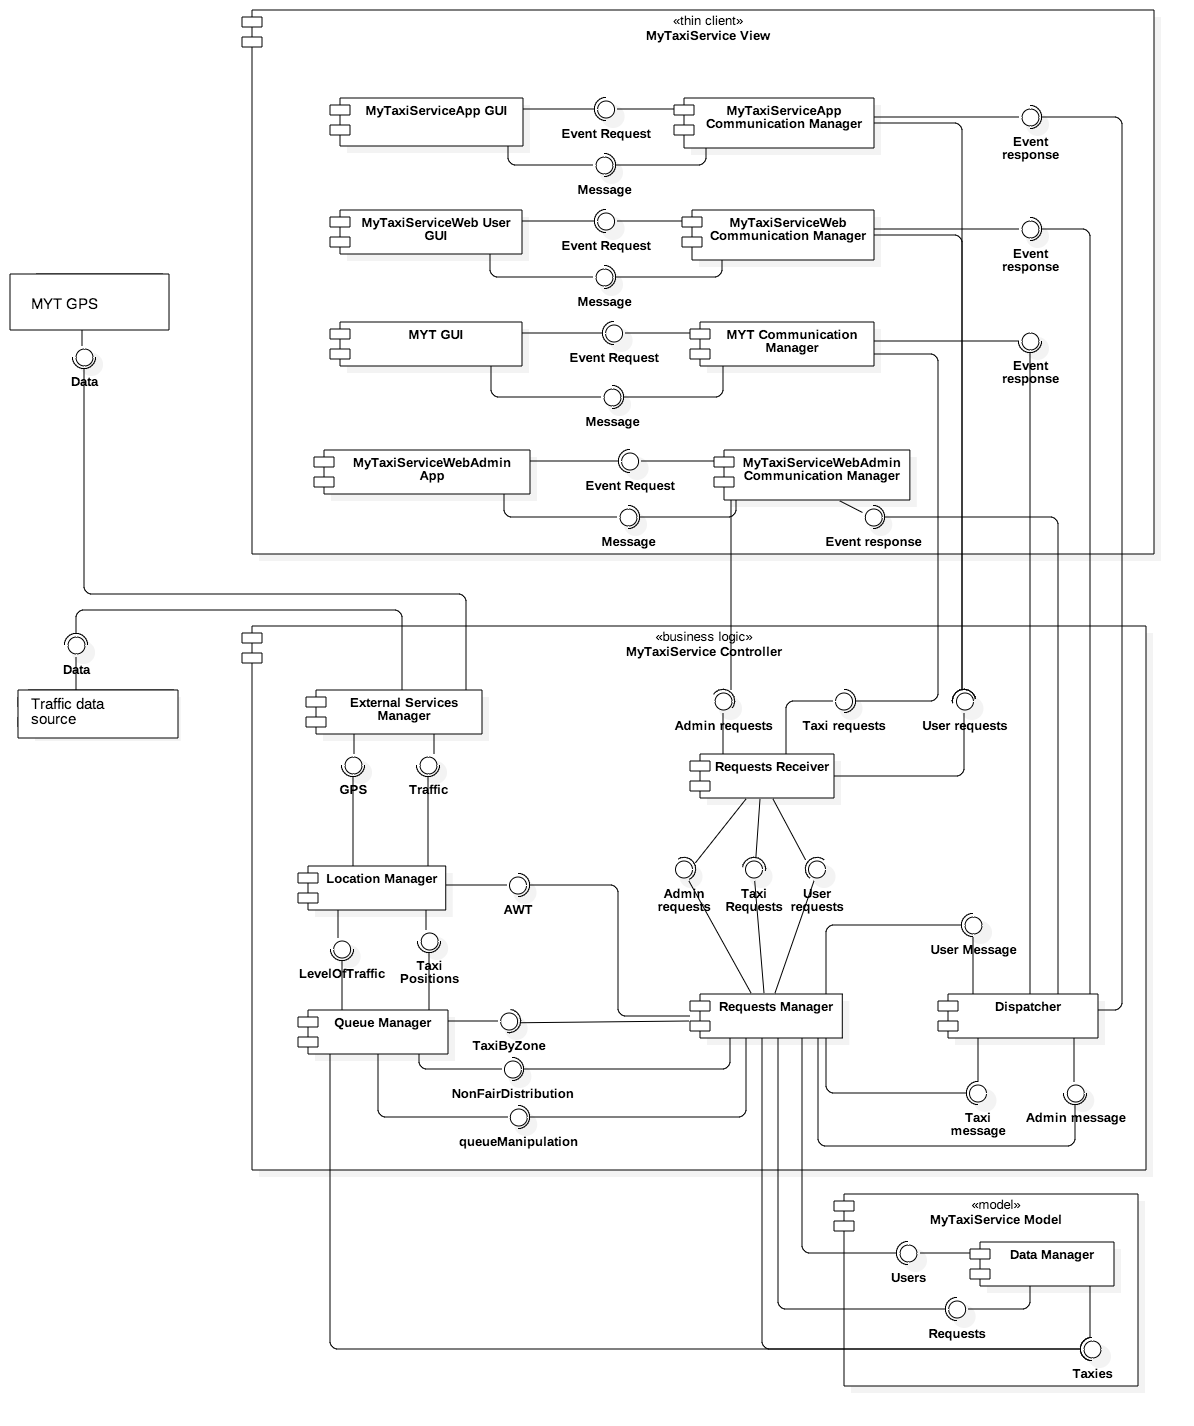
\includegraphics[scale=0.42]{component.png}
\end{changemargin}
\newpage
\subsection{Runtime View}
\begin{changemargin}{0cm}{0cm}{-2.5cm}
	Components interaction in case of ride request.\newline
	\noindent
	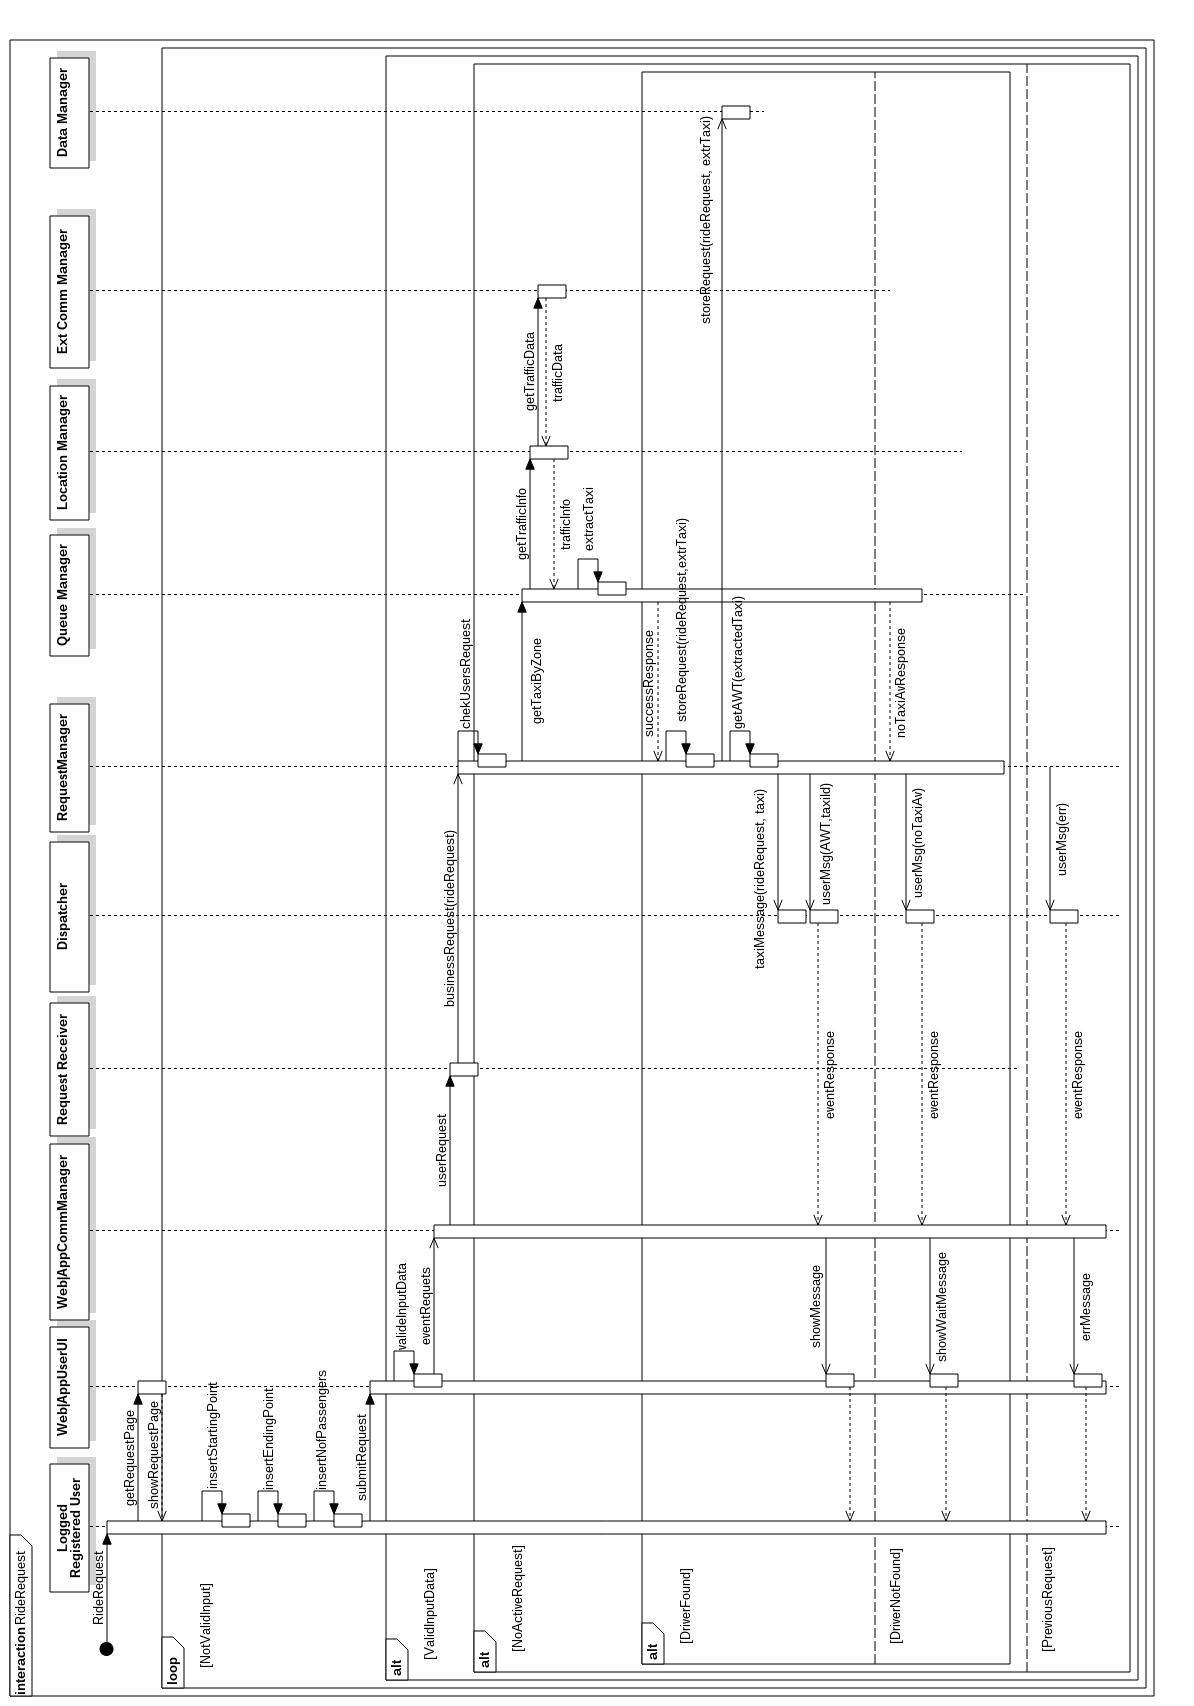
\includegraphics[scale=0.42]{sd1.png}
\end{changemargin}
\newpage
\begin{changemargin}{0cm}{0cm}{-2.5cm}
	Components interaction in case of booking request.\newline
	\noindent
	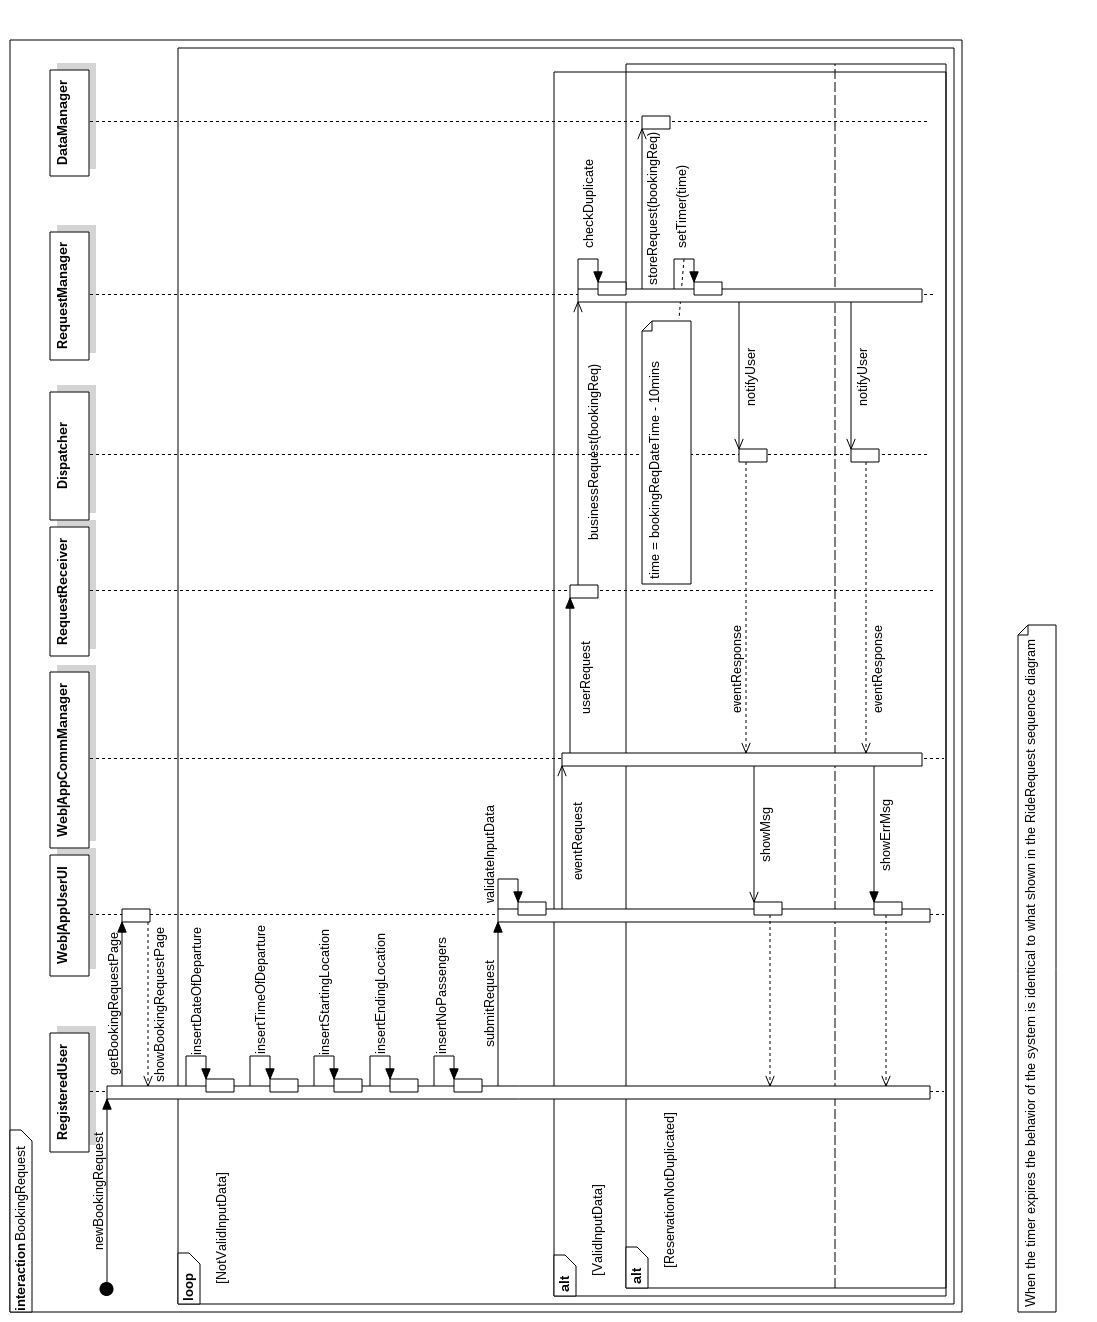
\includegraphics[scale=0.42]{sd2.png}
\end{changemargin}
\newpage
\begin{changemargin}{0cm}{0cm}{-2.5cm}
	Components interaction when a new taxies redistribution is needed .\newline
	\noindent
	\begin{minipage}{\linewidth}
	\makebox[\linewidth]{
	  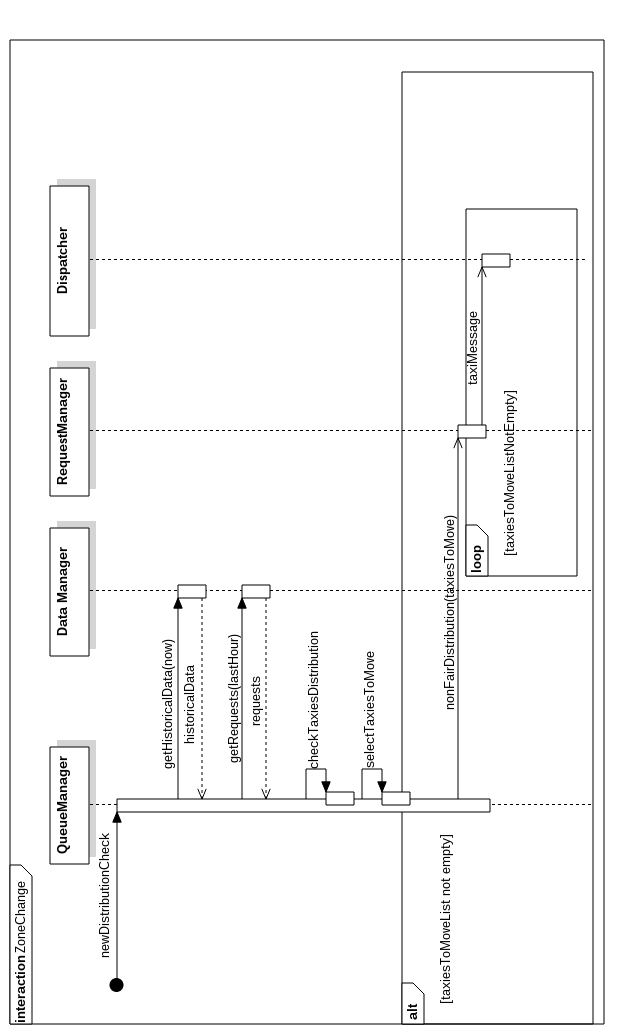
\includegraphics[scale=0.45]{sd3.png}}
	\end{minipage}
\end{changemargin}
\newpage
\begin{changemargin}{0cm}{0cm}{-2.5cm}
	Components interaction in case of user login.\newline
	\noindent
	\begin{minipage}{\linewidth}
	\makebox[\linewidth]{
	  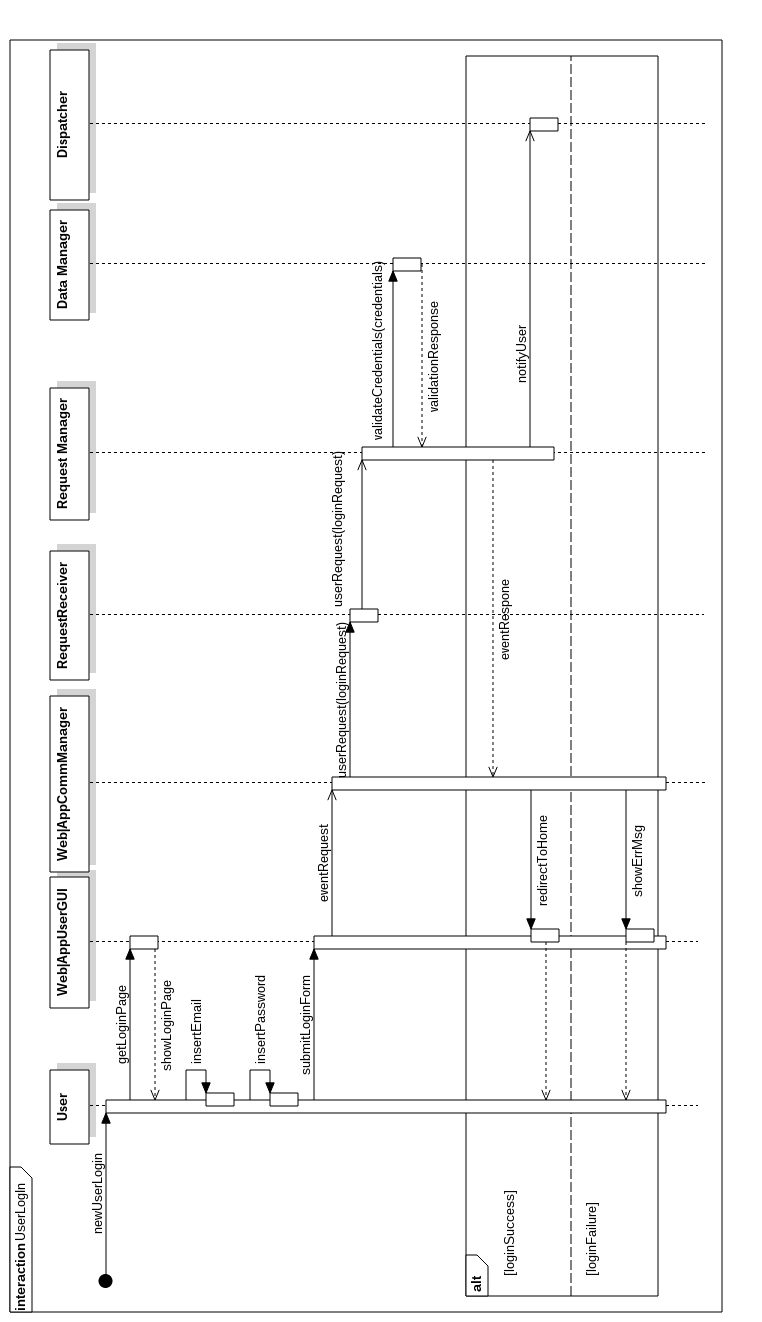
\includegraphics[scale=0.42]{sd4.png}}
	\end{minipage}
\end{changemargin}
\newpage
\begin{changemargin}{0cm}{0cm}{-2.5cm}
	Components interaction in case of accident notification from a driver.\newline
	\noindent
	\begin{minipage}{\linewidth}
	\makebox[\linewidth]{
	  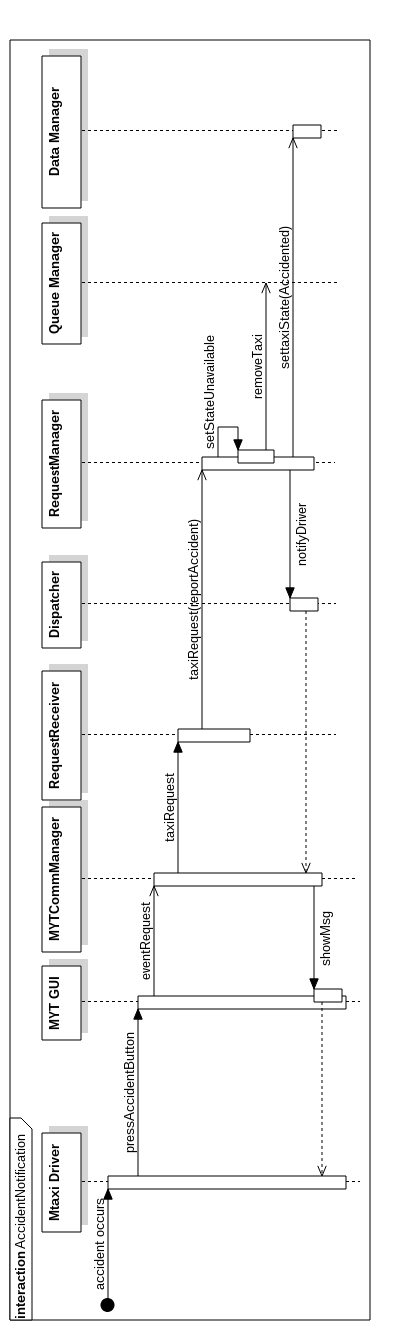
\includegraphics[scale=0.42]{sd5.png}}
	\end{minipage}
\end{changemargin}
\newpage
\begin{changemargin}{0cm}{0cm}{-2.5cm}
	Components interaction when the driver notify a ride end.\newline
	\noindent
	\begin{minipage}{\linewidth}
	\makebox[\linewidth]{
	  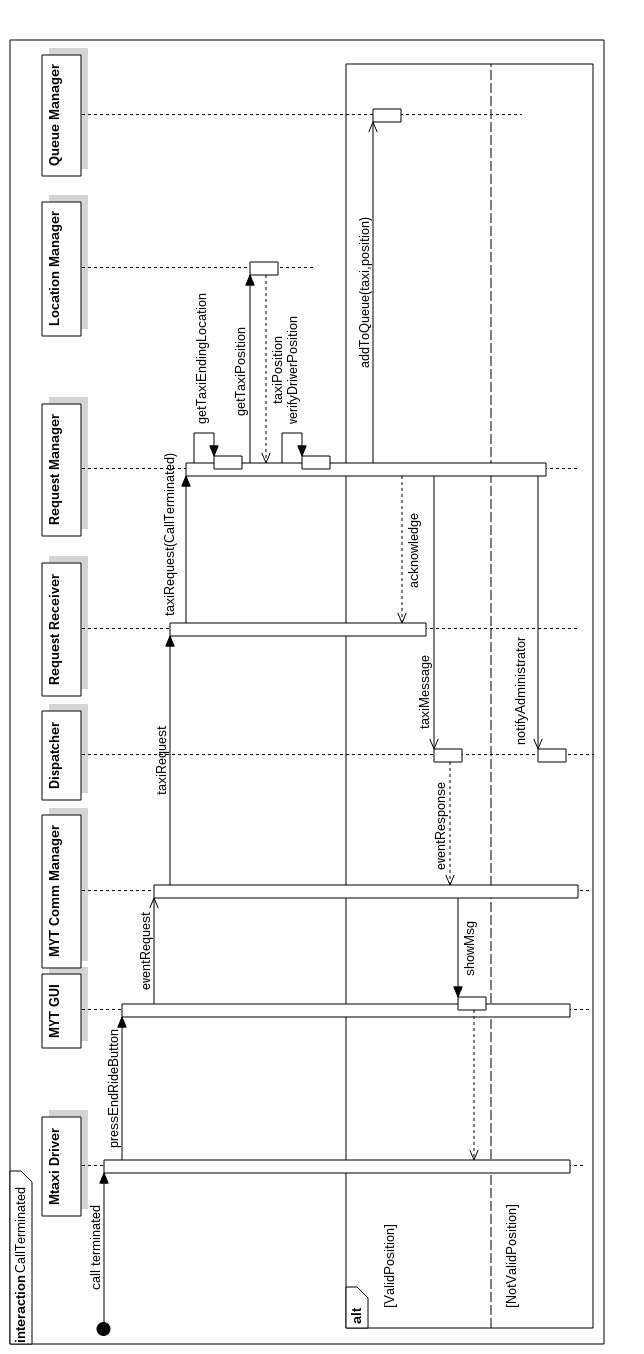
\includegraphics[scale=0.42]{sd6.png}}
	\end{minipage}
\end{changemargin}
\newpage
\begin{changemargin}{0cm}{0cm}{-2.5cm}
	Components interaction in case of user registration.\newline
	\noindent
	\begin{minipage}{\linewidth}
	\makebox[\linewidth]{
	  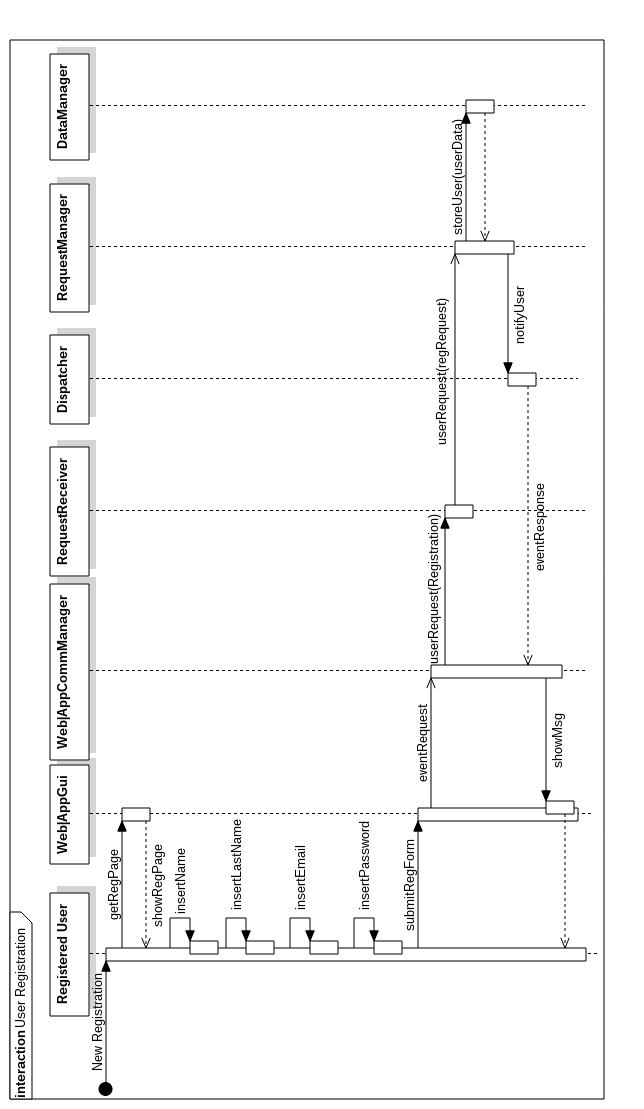
\includegraphics[scale=0.42]{sd7.png}}
	\end{minipage}
\end{changemargin}
\newpage

\subsection{Components Interface}
\begin{description}
     \item [Request Receiver] \hfill \\
          This component interfaces with the communication managers of the view in three ways: it receives and pre-process requests from users
          (users requests), from mtaxi drivers(taxies requests) and from
          administrators(admin requests). In addition to that, it
          directly communicates with the Request Manager so that the above  mentioned requests are
          fully elaborated and executed; this is done using three interfaces: one for other requests, another for business
          requests and last one for admin requests.
          All messages are exchanged in synchronous way on both side.

      \item [Request Manager] \hfill \\
          This components interfaces with all the components of the controller except for the External Services Manager, it also interfaces
          all the components of the model.
          In particular the Request Manager communicates with:
	\begin{enumerate}
	            \item Location Manager: via the AWT interface in order to get the AWT for a mtaxi to reach a user
	            (synchronous communication)
	            \item Queue Manager: via three interfaces:
		 \begin{enumerate}
		                \item TaxiByZone: in order to get the first available mtaxi for a given zone
		                (synchronous communication)
		                \item NonFairDistribution: the Request Manager observes the Queue Manager for a non fair distribution of mtaxies among city's zones and so for a set of mtaxies
		                the need to be moved to other specified zones
		                (asynchronous communication)
		                \item ManipulateQueue: in order to manipulate the mtaxies in a given queue (for example when a mtaxi reports and accident, then it should be
		                made non available and removed by its zone associated queue)
		                (synchronous communication)
		\end{enumerate}
	          \item Dispatcher: via three interfaces:\newline
		All the communications are synchronous
		\begin{enumerate}
	                \item Users messages : in order to send a response to a user request
	                \item Taxi messages : in order to send a response to a mtaxi request
	                \item Admin messages : in order to send a response to an admin request
		\end{enumerate}
	          \item Data Manager: via three interfaces:\newline
		All the communications are synchronous
		\begin{enumerate}
	               \item Users : in order to store/retrieve data about users
	               \item Taxies : in order to store/retrieve data about mtaxies
	               \item Requests : in order to store/retrieve data about requests
		\end{enumerate}
     \end{enumerate}
      \item [Queue Manager] \hfill \\
          This components offers to the Request Manager the interfaces already described above. In addition to that
          it communicates with:
	\begin{enumerate}
	          \item Location manager : via two interfaces:\newline
		All the communications are asynchronous
		\begin{enumerate}
		            \item Taxi positions: in order to get the position(in terms of city zone) of mtaxies
		            \item LevelOfTraffic : in order to get the level of traffic for a mtaxi and so use another mtaxi
		            to fullfill a request
		\end{enumerate}
	          \item Data Manager via an already considered interface:
		\begin{enumerate}
	           	\item Taxies : in order to retrieve data about mtaxies and populate the zone per zone queues
		\end{enumerate}
	\end{enumerate}

       \item [Data Manager] \hfill \\
          This component offers to the Request Manager the interfaces already described above to retrieve/store data
          from to the database

      \item [Location Manager] \hfill \\
          This component offers to the Request Manager and to the Queue Manager the interfaces already described above. In addition to that it communicates
          with the External Services Manager via two interfaces:\newline
	All the communications are synchronous
	\begin{enumerate}
	          \item GPS : in order to get raw gps data from mtaxies thanks to to GPS system integrated in their MYT
	          \item Traffic : in order to get raw data about the traffic from a generic external provider
	\end{enumerate}

      \item [Dispatcher] \hfill \\
          This component offers to the Request Manager the interfaces already described above.
          In addition to that, it communicates(indirectly using the web) with the communication managers of the view
          via the event response interfaces; this is done in order to deliver responses to requests and to deliver asynchronous messages
          (asynchronous and synchronous communication)

      \item [External Services Manager] \hfill \\
          This component offers to the Location Manager the interfaces already described aboive.
          In addition to that, it communicates with:
	\begin{enumerate}
	          \item The MYT device GPS system via the data interface; this is done in order to get the gps coordinates of a mtaxi
	          \item A generic traffic source via the data interface; this is done in order to get raw data about the traffic
	          conditions of the city
	\end{enumerate}
          All communications are asynchronous

      \item [MyTaxiServiceApp/MyTaxiServiceUserWeb/MyTaxiServiceAdminWeb/MYT GUI] \hfill \\
          These components offers to their relative communication managers a message interface
          They communicate with their relative communication managers via the event request interface; this is
          done in order to forward a generic request to MyTaxiService(B)
          All communications are synchronous

      \item [MyTaxiServiceApp/MyTaxiServiceWeb/MYT/MyTaxiServiceAdminWeb Comm. Manager] \hfill \\
          These components offers to the Dispatcher the already described interfaces. In addition to that
          they communicate with the relative GUIs using the message interfaces; this is done in order
          to make the GUI display a response to a request or an asynchronous message
          All communications are asynchronous

\end{description}

\subsection{Selected architectural styles and patterns}
        Some important preliminary considerations:
        \begin{itemize}
	        \item The number of requests and of users could be very high
	        \item In the future MyTaxiService can be made available for other cities
	        \item The number of requests can have a very high variance(e.g if an important event is held in the city then the number
	        of requests will probably increase by a lot)
         \end{itemize}

        Due to these simple considerations the chosen architecture for MyTaxiService is a 3 tiers Client/Server architecture.
        This kind of architecture has been chosen because it guarantees:
        \begin{itemize}
	        \item Scalability: the nodes that compose the application server and db server can be increased in number without the need
	        of redesign the whole system
	        \item Reliability: since the chosen architecture is distributed, failures can be isolated easily and db replications can be
	        implemented without impacting too much on the design of the whole system
	        \item Adaptability: the chosen architecture can easily be enriched with a load balancer that distributes and activates nodes
	        in relation to the number of incoming requests
	        \item Security: since the chosen architecture divides strictly business logic and data and since the application server
	        and the db server are isolated from the web using firewalls, malicious attacks can be prevented and high level of
	        security granted
	\end{itemize}


        The chosen architecture composes of:
         \begin{enumerate}
	          \item A tier(view) which include:
		\begin{enumerate}
		            \item Smartphones in which the MyTaxiService mobile app is installed
		            \item Smartphones and computers trough which MyTaxiService User website is accessible
		            \item Smartphones and computers trough which MyTaxiService Admin website is accessible
		            \item MYT devices trough which mtaxi drivers can manage ride requests
		\end{enumerate}

	          \item A tier(controller) that is composed by an application server(can be distributed) that manages requests coming from users
	          and mtaxies by applying the bussines logic at the base of the whole system
	          \item A tier that is composed by a database server(can be distributed) that manages data manipulation and access requests from
	          the system's application server
	          \item A set of external services used by the application server to implement part of its logic. It is supposed that these
	          services are distributed to the system using a SOA architecture.
	\end{enumerate}
	The websites assets are hosted by a webserver.\newline

        The client in this architecture is a "thin" client, it just contains only an interaction/visualization layer, all
        the logic of the application is condensed in the application server, which is, in this way, a "fat" server.\newline


        As already mentioned above the central system makes use of external service regarding the traffic information in the
        city. It could be assumed that information are distributed to MyTaxiService via a SOA architecture because this is
        the most suitable(and most used) way to distribute data and services to external companies.\newline

        \textbf{The role of polling}\hfill \\
        The business logic behind the system demands that users and mtaxies don't  receive information only as a response to a request, but
        also as a non requested message from MyTaxiService(B). Mantaining a continuosly opened connection between the client and the application server
        seems not an efficient and sustainable strategy, so is assumed that users and mtaxies checks periodically if MyTaxiService(B) has any messages
        for them. This strategy is known as polling.\newline
        \newpage
        Follows a schematic diagram of the system architecture:\newline
        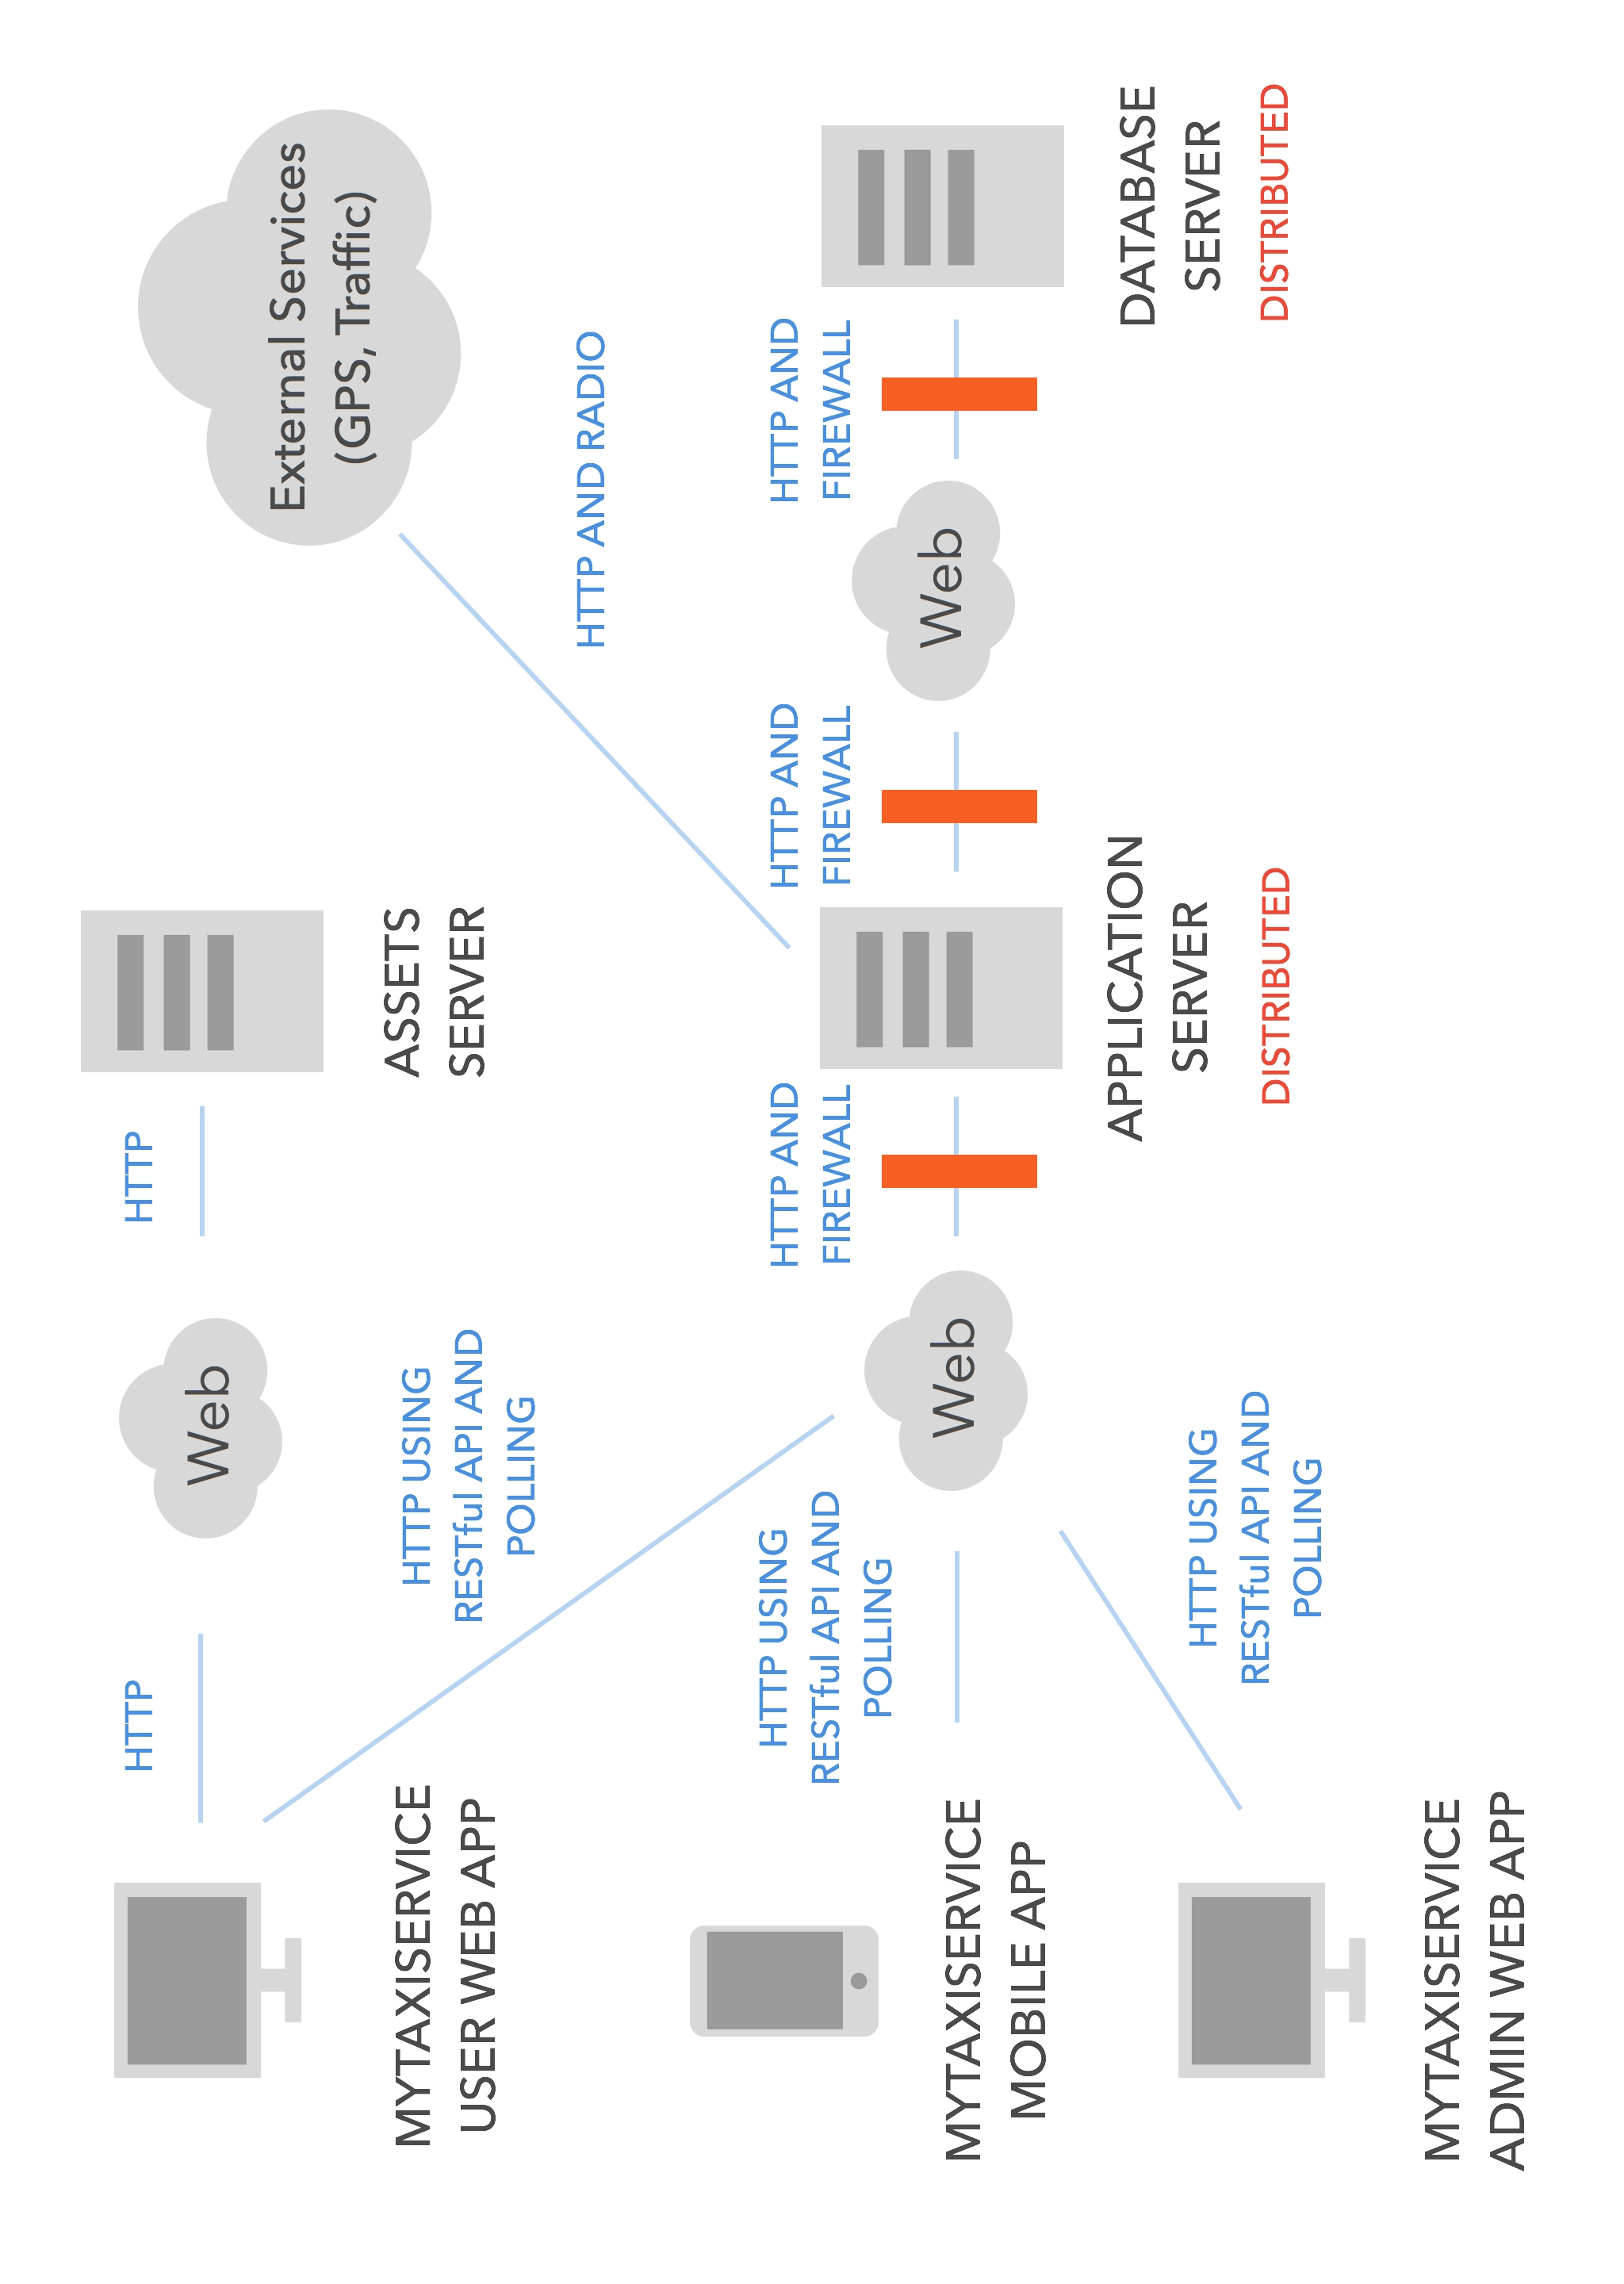
\includegraphics[scale=0.3]{Arch.jpg}
 
\newpage

\subsection{Deployment View}
In this section is included a deployment diagram showing how high level components are mapped on the architecture tiers.\newline
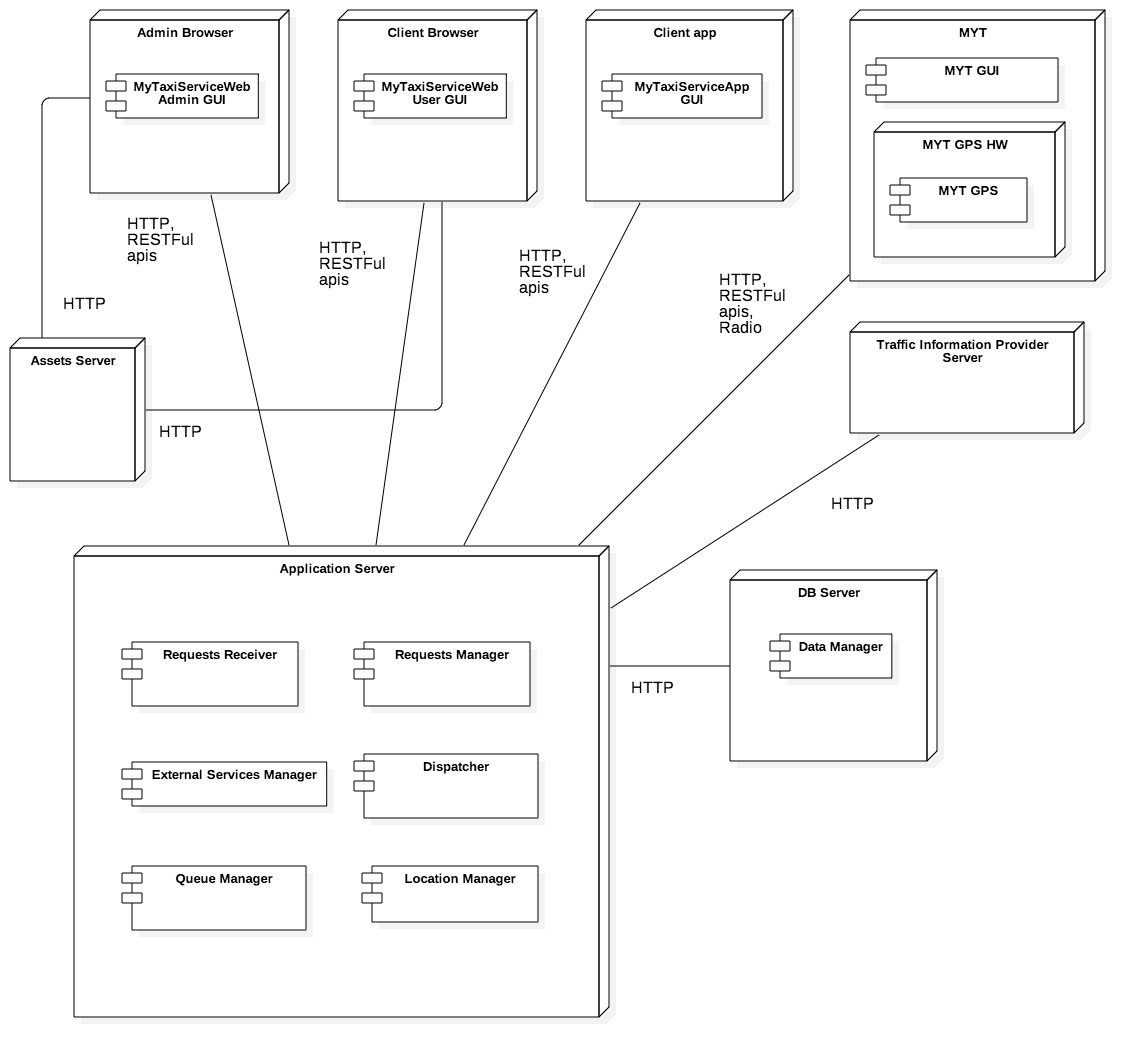
\includegraphics[scale=0.4]{deployment.png}

\newpage

\section{Algorithms Design}
The following algorithm is run in the Queue Manager component periodically(each hour).
  Its objective is to try to reditribute taxies present in the city's zones in order
  to match the expected demand of taxies in each zone.
  To accomplish this objective the first part of the algorithm computes, for each zone,
  the expected demand by means of the following formula:\newline

    $ expectedTaxies = ((historicalAvg*w1+currentAvg*w2)*zone.getWeight()) $\newline

  This formula is based both on historical data for the current day and time and
  the last hour data registered in the database.
  Each of this two terms is "weighted" (w1,w2) in order to determine how
  the old and new data contributes to the final result.
  The above formula takes also into account the size of the by means of a third
  weight typical of each zone(zone.getWeight()), the more the value is near to 1
  the more the zone is bigger. This is necessary to consider the fact that smaller
  zones in general have a smaller number of request wrt to bigger zones.
  For each zone the number of taxies already present is subtracted from the
  expectedTaxies value(for that zone). This operation produces the taxiesToMove
  variable that if positive indicates a zones that has a "surplus" of taxies and
  if negative indicates a zone with a "deficit" of taxies.
  Queues are then divided into two separated lists(surplusQueues, deficitQueues)
  according to the value of taxiesToMove.
  The lists are sorted according to the value of taxiesToMove.
  The algorithm reditribute the taxies by initially considering the couple of queues which
  has the highest number of taxies in respectively in deficit/surplus.
  The algorithm proceeds by selecting queues with deacreasing number of taxiesToMove.
  The function return when:
\begin{itemize}
    \item The expected demand of taxies has been fullfilled
    \item There are no more taxies to fullfill the expected demand
\end{itemize}
\begin{lstlisting}
// 0 < w1, w2 < 1
function computeDistribution(float w1, float w2) {
  /*The following for cycle computes, for each zone, the number of taxies
   *required(taxiesToMove < 0) or the number of taxies in surplus(taxiesToMove > 0)
   */
  foreach(zone in zones){
    //Get the average number of requests for the current day/hour
    historicalAvg = getHistData(now.date, now.hour, zone);
    //Get the number of requests registered in the last hour
    currentAvg = getLastHourData(zone);
    //Computes the expected number of taxies required in this zone for the following hour
    taxiesToMove = ((historicalAvg*w1+currentAvg*w2)*zone.getWeight())/2 - zone.getTaxies();
    //Assigns the expected number of taxies to the relevant queue
    zone.getQueue().setTaxiesToMove(taxiesToMove);
  }

  //surplusQueues is the list of queues that has some taxies to offer
  surplusQueues = [/*List of queues with taxiesToMove > 0*/];
  //deficitQueues is the list of queues that requires some taxies
  deficitQueues = [/*List of queues with taxiesToMove < 0*/];

  //Sort surplusQueues by deacreasing taxiesToMove
  Sort(surplusQueues);
  //Sort deficitQueues by deacreasing taxiesToMove
  Sort(deficitQueues);

  //i iterates over surplusQueues
  //j iterates over deficitQueues
  while(i < surplusQueues.length  && j < deficitQueues.length){

    //If the current surplusQueues has more taxies to offer than the current deficitQueues
    if(surplusQueues[i].getTaxiesToMove > deficitQueues[j].getTaxiesToMove){
      deficitQueues[j].setTaxiesToMove(0);
      surplusQueues[i].setTaxiesToMove(oldValue-deficitQueues[j].getTaxiesToMove);
      //Select the next deficitQueues
      j++;
      //Send the order
      foreach(taxi in surplusQueues[i].getTaxies()) {
        moveTaxi(deficitQueues[j],taxi)
      }

    }
    //If the current deficitQueues reuires more than what the current surplusQueues has to offer
    else if(surplusQueues[i].getTaxiesToMove < deficitQueues[j].getTaxiesToMove){
      serplusQueues[i].setTaxiesToMove(0);
      deficitQueues[j].setTaxiesToMove(oldValue-surplus[j].getTaxiesToMove);
      //Send the order
      foreach(taxi in surplusQueues[i].getTaxies()) {
        moveTaxi(deficitQueues[j],taxi)
      }
      //Select the next surplusQueues
      i++;
    }
    //If the current deficitQueues requires exaclty what the current surplusQueues offers
    else{
      serplus[i].setTaxiesToMove(0);
      deficit[j].setTaxiesToMove(0);
      //Send the order
      foreach(taxi in surplusQueues[i].getTaxies()) {
        moveTaxi(deficitQueues[j],taxi)
      }

      //Select the new surplus/deficitQueues
      i++;
      j++;
    }
    deficitQueuesurplusQueues[i].getTaxiesToMove
  }
}

/* Adds taxi to endingQueue
 * Sends a change zone order to taxi via a primitive provided by
 * the Request Manager component
 */
function moveTaxi(endingQueue, taxi) {
  endingQueue.add(taxi);
  sendChangeOrder(taxi);
}

\end{lstlisting}
Following several graphs showing the evaluation of the expectedTaxies function in three different situations:\newline
\begin{changemargin}{-2cm}{0cm}{0cm}
	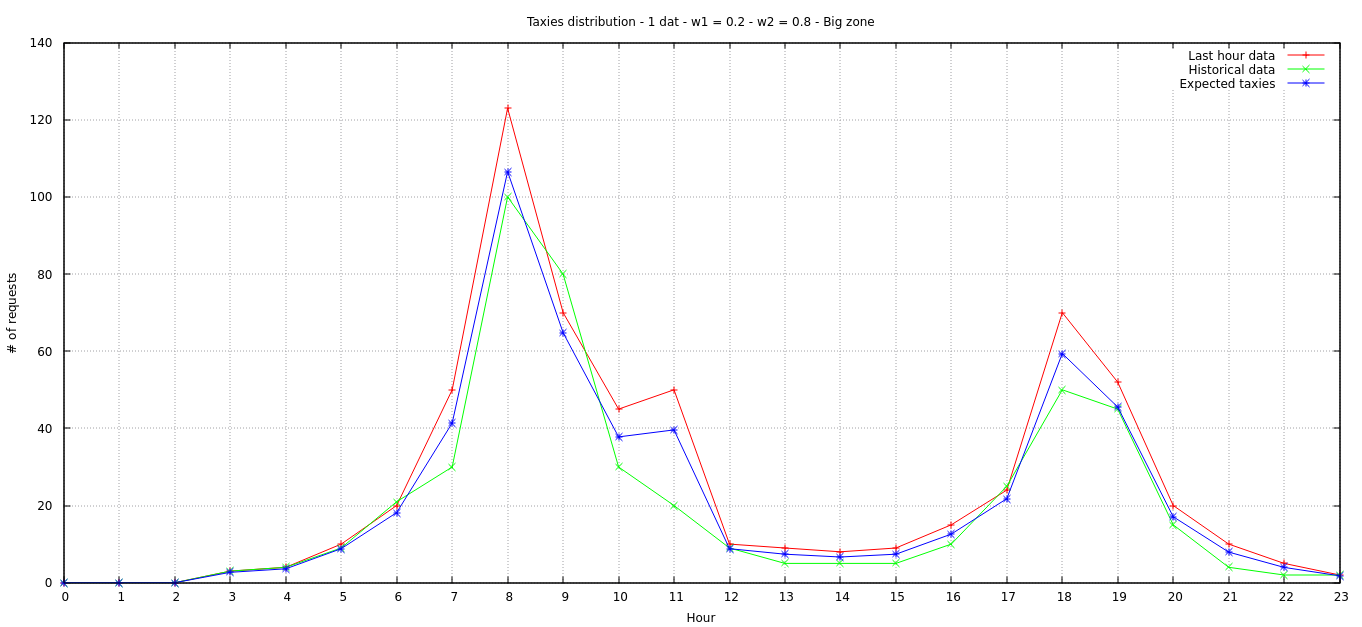
\includegraphics[scale=0.5]{graph1.png}
	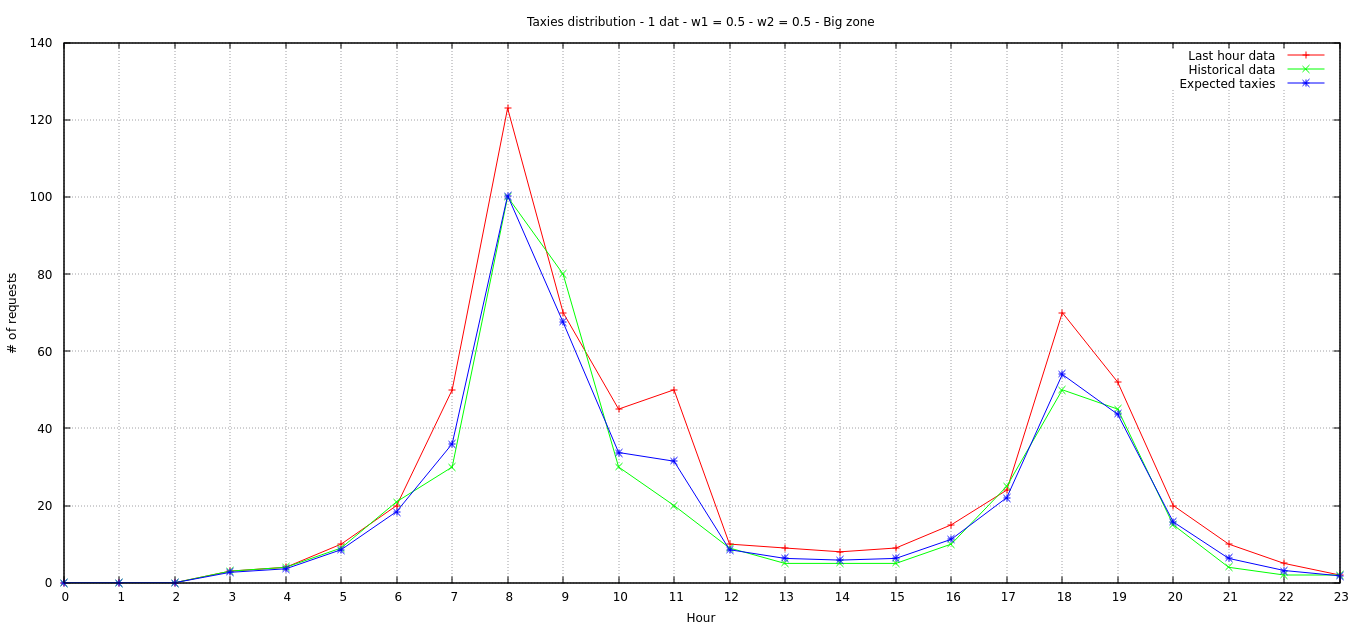
\includegraphics[scale=0.5]{graph2.png}
	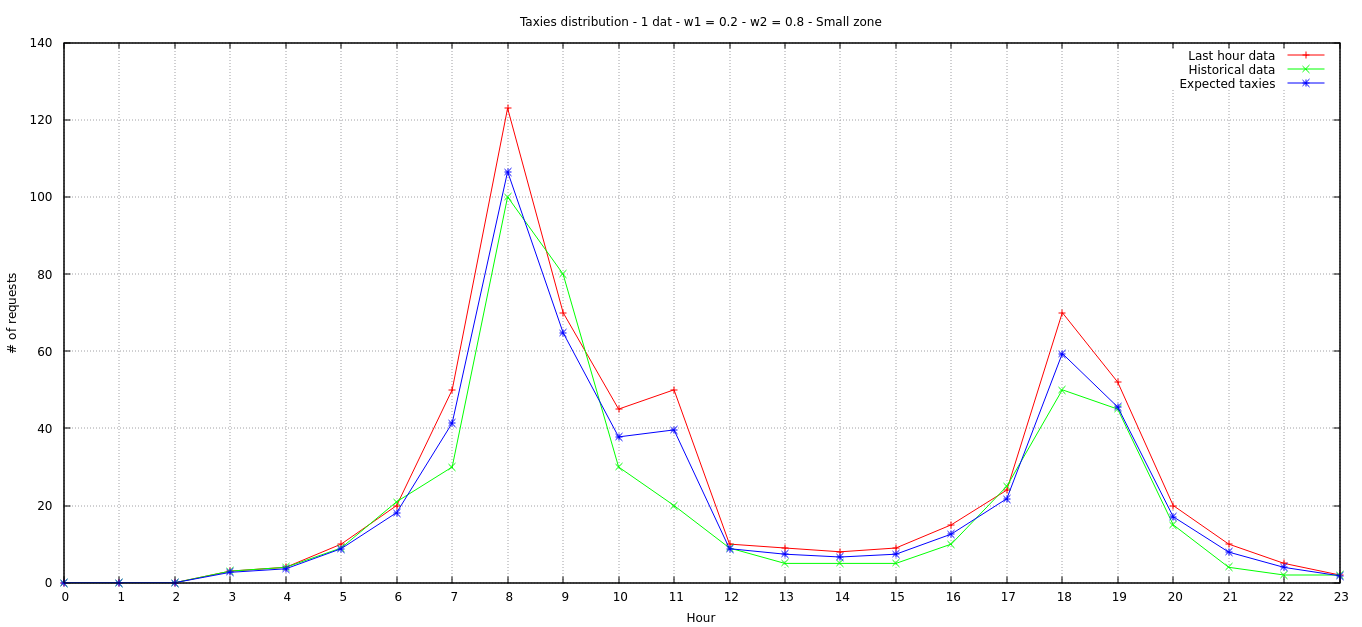
\includegraphics[scale=0.5]{graph3.png}
\end{changemargin}
\newpage
\section{User Interface Design}
	No new useful user interface needs to be specified in this section.\newline
	For a detailed description of the user interfaces, please refer to section 2.2.2 of the RASD v1.1 document.

\newpage
\section{Requirements Traceability}
	\begin{table}[h]
		\centering
		\begin{tabular}{|| c || c ||}
			\hhline{|t:==:t|}
  			\textbf{Component} & \textbf{Requirements} \\
			\hhline{|:=|=:|}
 			Dispatcher & (32)  (34) (42)\\
			\hhline{|:-|-:|}
 			Request Manager &  (1a) (2a) (2b) (3a) (3b) (3c) (3e) (4a) (6) (15) (29) (34) (42)\\
			\hhline{|:-|-:|}
 			External Services Manager &  (19) (20)\\
			\hhline{|:-|-:|}
 			Location Manager & (19) (20) (26) (30) (41) (42)\\
			\hhline{|:-|-:|}
 			Queue Manager &  (27) (28) (31) (33) (39)\\
			\hhline{|:-|-:|}
 			Request Receiver &  \\
			\hhline{|:-|-:|}
 			Data Manager &  (1a) (2a)(3b) (3c) (4a) (37) (38) \\
			\hhline{|:-|-:|}
 			&  \\
			\hhline{|:-|-:|}
 			&  \\
			\hhline{|:-|-:|}
 			&  \\
			\hhline{|:-|-:|}
			&  \\
			\hhline{|b:==:b|}
		\end{tabular}
		\caption{Requirements Traceability matrix}
\end{table}

\end{document}
